\documentclass[a4paper]{article}

\usepackage[english]{babel}
\usepackage[utf8]{inputenc}
\usepackage{fullpage}
\usepackage{amsmath}
\usepackage{graphicx}
\usepackage[colorinlistoftodos]{todonotes}
\usepackage{hyperref}
\usepackage{amssymb}
\usepackage{outline} 
\usepackage{pmgraph} 
\usepackage[normalem]{ulem}
\usepackage{graphicx}  % Lets you insertPDF images
\usepackage{svg}  % Lets you insert svg images
\usepackage{verbatim}
\usepackage{afterpage}  % new pages

% Notes
\usepackage{todonotes}

% Tikz drawings
\usetikzlibrary{matrix, backgrounds, fit}

% Colored text
\usepackage{xcolor}

% Bold mathematical expressions
\usepackage{fixmath}

% Confusion Matrix
\usepackage{array}
\usepackage{multirow}
\newcommand\MyBox[2]{
  \fbox{\lower0.75cm
    \vbox to 1.7cm{\vfil
      \hbox to 1.7cm{\centering \hfil\parbox{0.5cm}{#1\\#2}\hfil}
      \vfil}%
  }%
}

% Lorem Ipsum
\usepackage{lipsum}

% Tables
\usepackage{array}
\newcolumntype{C}[1]{>{\centering\arraybackslash}m{#1}}

\newcommand{\homeCOne}{../../Chapter 1 - Metalabeling/Draft}
\newcommand{\homeCTwo}{../../Chapter 2 - FracDiff/Draft}

% ____ Bibliography ____
\usepackage{natbib} %Bibliography.
% \setcitestyle{numbers} %Cite as numbers or author-year.
\bibliographystyle{plain} %Reference style.
% ______________________

\begin{document}
\begin{titlepage}
  \centering
  \sc \LARGE

  \rule{\textwidth}{1.6pt}\vspace*{-\baselineskip}\vspace*{2pt}
  \rule{\textwidth}{0.4pt}
  \vspace{-6mm}

  \textbf{Draft - Chapter 1: Meta-labeling}\\[1.25ex]

  \vspace{-3.5mm}
  \rule{\textwidth}{0.4pt}\vspace*{-\baselineskip}\vspace*{3.2pt}
  \rule{\textwidth}{1.6pt}
  \vfill

  \Large
 \centering{Author: Guillermo Creus Botella} \\

  \Large
  Supervisor: Daniel P. Palomar
  \vfill

  \includegraphics[height=3.5cm]{img/hkust.png} \hspace{2.5cm}
  \includegraphics[height=3.5cm]{img/upc.png}
  \vspace{1cm}

  \textit{The Hong Kong University of Science and Technology} (HKUST)\\
  \vspace{1cm}
  \textit{Polytechnic University of Catalonia - BarcelonaTech} (UPC)\\
  \vfill

\end{titlepage}

\pagenumbering{arabic}
\null
\thispagestyle{empty}
\addtocounter{page}{-3}
\newpage

\thispagestyle{empty}
\tableofcontents

\newpage\null\thispagestyle{empty}\newpage

\section{Stationary Time Series}
\label{sec:stationaryTimeSeries}
What should be covered:
\begin{itemize}
	\item Stationary financial time series are really important

	\item Definition of stationarity
\end{itemize}

\vspace{2cm}

% _____ References _____

% https://www.wne.uw.edu.pl/files/2116/0190/5073/WNE_WP338.pdf

% Signal efficacy - Hudson Thames - Metalabeling

%Tsay - Analysis of Financial time series

%Heino Bohn Nielsen. "Non-Stationary Time Series and Unit Root Tests" (PDF).
%http://web.econ.ku.dk/metrics/Econometrics2_05_II/Slides/
%08_unitroottests_2pp.pdf

%  @Manual{,
%    title = {tseries: Time Series Analysis and Computational Finance},
%    author = {Adrian Trapletti and Kurt Hornik},
%    year = {2019},
%    note = {R package version 0.10-47.},
%    url = {https://CRAN.R-project.org/package=tseries},
%  }

%Hosking, J (1981): “Fractional differencing.” Biometrika, Vol. 68, No. 1, 
%pp. 165-175.

% _______________

A time series $\{x_t\}$ is said to be \textbf{strictly stationary} 
if the joint distribution of $(x_{t_1},\ \ldots ,\ x_{t_k})$ is the same as 
the one of $(x_{t_1 + t},\ \ldots ,\ x_{t_k + t})\ \forall t$ and 
$\forall (t_1,\ \ldots,\ t_k)$ where $k \in \mathbb{N}$. That is, the joint 
distribution is time invariant.\\

However, as this definition of stationarity is complicated to verify 
empirically, a new definition will be introduced. That being said, a time 
series is said to be \textbf{weakly stationary} if:

\begin{enumerate}
	\item $\mathbb{E}[x_t] = \mu = \text{ct.}$
	\item $\text{Cov}[x_t,\ x_{t-l}] = \gamma_{l}$, which 
	only depends on the lag $l$.
\end{enumerate}

With that said, let's present an Autoregressive model of order $p$, AR(p):

\begin{align*}
	x_t = \sum_{i = 1}^{p} \theta_i x_{t-i} + \epsilon_t\\
	x_t = \sum_{i = 1}^{p} \theta_i B^i \ x_{t} + 
	\epsilon_t\\
	\phi(B) x_t = \epsilon_t 
\end{align*}

Where $B$ is the backshift operator ($B x_t = x_{t-1}$). 
Additionally, the process will have a unit root (integrated of order 1 - 
$I(1)$) when $z = 1$ is a root of multiplicity 1 of the characteristic 
equation: $\phi(z) = 1 - \theta_1 \cdot z^1 -\ \ldots \ - \theta_p \cdot z^p 
= 0$. When $z = 1$ is a root of multiplicity $r$, the process is integrated 
of order $r$ - $I(r)$.\\

\textbf{In order to be weakly stationary, the roots of the polynomial $\phi$ 
must lie outside the unit circle, i.e., $|z_i| > 1$}\\

Rewriting everything:
\begin{align*}
	x_t - x_{t-1} = \left(\sum_{i = 1}^p \theta_i - 1 \right)
	x_{t-1} + \left(\sum_{i = 2}^p \theta_i \right) \cdot 
	(x_{t-2} - x_{t-1}) +\ \ldots +\ \theta_p \cdot 
	(x_{t-p} - x_{t-(p-1)}) \\
	\Delta x_t = \pi \cdot x_{t-1} + c_1 \cdot 
	\Delta x_{t-1} +\ \ldots +\ c_{p-1} \cdot 
	\Delta x_{t-(p-1)}
\end{align*}

Where $\pi = \sum_{i = 1}^p \theta_i -1$ and $c_j = - \sum_{i = j+1}^p 
\theta_i$\\

Noting that $\phi(1) = -\pi$, then $z = 1$ is a unit root if $\pi = 0$. 
Consequently, the Augmented Dickey-Fuller test is defined:

\begin{align*}
	H_0 : \pi = 0\\
	H_a : \pi < 0
\end{align*}

At this point, if a time series has no unit root, then $H_0$ will be 
rejected and it will be concluded that the time series is stationary.\\

Regarding the order $p$ of the AR model, the package \textbf{tseries} will 
be used, which sets $p = \lfloor \sqrt[3]{\text{T} - 1} \rfloor$ (T  = 
length of the time series - $x_1 ,\ \ldots ,\ x_\text{T}$) 
as default. This value of $p$ corresponds to the suggested upper bound on 
the rate at which the number of lags should be made to grow with the sample 
size for the general ARMA(p,q) setup.\\ %cite here

\section{Fractional differentiation}
\label{sec:fracDiff}
It is often the case that the original log-prices time series $y_t$ is non-
stationary. To mend that, a differentiation of order 1 is computed and the 
final time series $x_t = (1 - B) y_t = y_t - y_{t-1}$ is usually stationary. 
However, in the process, the ``memory'' of the time series is erased (see 
figure \ref{fig:tSeriesMemory}).\\

\begin{figure}[hbtp]
\centering
	\includegraphics[scale=0.5]{"\homeCTwo/img/tSeriesMemory"}
	\caption{Memory of differentiated series}
	\label{fig:tSeriesMemory}
\end{figure}

That is when fractional differentiation comes into play. It consists of 
defining the differentiated time series as $x_t^d = (1 - B)^d y_t$, 
$d \in (0,1)$, where:

\begin{align*}
	(1 - B)^d = \sum_{k = 0}^{\infty} \binom{d}{k} (-B)^k = 
	\sum_{k = 0}^{\infty} \frac{\prod_{i = 0}^{k - 1} (d - i)}{k!}\\
	= \sum_{k = 0}^{\infty} B^k (-1)^k \prod_{i = 0}^{k - 1} 
	\frac{d - i}{k - i} = \sum_{k = 0}^{\infty} w_k B^k
\end{align*}

Note that:
\begin{itemize}
	\item $w_k = -w_{k - 1} \cdot \frac{d - (k - 1)}{k}$ and $w_0 = 1$. See 
	figure \ref{fig:weightsD}. 
	\item $d = 1 \Rightarrow x_t^1 = y_t$ - log-prices
	\item $d = 0 \Rightarrow x_t^0 = x_t$ - log-returns
\end{itemize}

\begin{figure}[htbp]
\centering
	\includegraphics[scale=0.5]{"\homeCTwo/img/weightsD"}
	\caption{Weights as a function of d}
	\label{fig:weightsD}
\end{figure}

% cite DePrado!!!!!
Before starting to differentiate the time series, a technique called 
``Fixed-width window fractional differentiation'' (FFD) will be defined. The 
purpose of this technique is to allow all the observations to have the same 
amount of memory. Because of data limitations, fractional differentiation 
can not be computed on an infinite series of weights. That is, $x_T^d$ will 
use $w_0,\ \ldots , w_{T - 1}$, while $x_{T - l}$ will use 
$w_0,\ \ldots , w_{T - l - 1}$.\\

Consequently, some observations will have more ``memory'' than others, which 
is not something one wants. Thus, by setting a threshold
(e.g., $\tau = 10^{-4}$), the following set of weights can be defined:

\begin{equation*}
	\tilde{w}_k =
	\begin{cases}	 
		w_k & \text{if } k \leq l^*\\
		0 & \text{if } k > l^*\\
	\end{cases}
\end{equation*}

Where $l^*$ is such that $|w_{l^*}| > \tau$ and $|w_{l^* + 1}| \leq \tau$. 
Note that the differentiation will be valid only for $t \geq l^* + 1$ and 
the same set of weights, $\{w_{k}\}_{k = 0}^{l^*}$, will be used for all 
estimates.\\

Finally, by setting a fixed $\tau$, the FFD differentiation can be 
expressed as:

\begin{equation}
	\label{eqn:FFD}
	x_t^d = \sum_{k = 0}^{\infty} \tilde{w}_k B^k y_t = \sum_{k = 0}^{l^*} 
	\tilde{w}_k B^k y_t \equiv \phi_d \ y_t \ \ (t \geq l^* + 1)
\end{equation}

To clarify everything, figure \ref{fig:FFD} shows $x_t^d$ for different 
values of $d$.\\

\begin{figure}[htbp]
\centering
	\includegraphics[scale=0.5]{"\homeCTwo/img/FFD"}
	\caption{FFD time series - $\tau = 10^{-4}$}
	\label{fig:FFD}
\end{figure}

Now that the corresponding $x_t^d$ time series have been computed, it is 
relevant to introduce again the ADF test. The objective is to find the 
minimum $d$, $d^*$, such that one can conclude that $x_t^{d^*}$ is 
stationary. In figure \ref{fig:ADFFFD}, the ADF test statistic is shown 
(using lag $p = \lfloor \sqrt[3]{\text{T}_d - 1} \rfloor$).\\

\begin{figure}[htbp]
\centering
	\includegraphics[scale=0.5]{"\homeCTwo/img/ADFFFD"}
	\caption{ADF statistic for FFD time series (p-value = 0.01)}
	\label{fig:ADFFFD}
\end{figure}

Figure \ref{fig:ADFFFD} also shows that int order to pass the ADF test, and 
conclude that the time series is stationary, $d = 0.2$ is sufficient.

\subsection{Inverse of differentiation}
\label{sec:invDiff}
In this section, the inverse of differentiation will be introduced since it 
is useful to go from one time series to the other. First of all, for 
convenience, let's define $x_t^d$ for $1 \leq t \leq l^*$:

\begin{equation}
\label{eqn:xDiffAdapted}
	x_t^d =
	\begin{cases}
		\phi_d (y_t) & \text{if } t \geq l^* + 1\\
		 \sum_{k = 0}^{t - 1} \tilde{w}_k \cdot B^k (y_t) & \text{if } 
		 1 \leq t \leq l^*
	\end{cases}
\end{equation}

Alternatively, if one defines $y_t = 0$ for $-l^* \leq t \leq 0$, equation 
\ref{eqn:xDiffAdapted} can be expressed as:

\begin{equation*}
	x_t^d = \phi_d (y_t) \ \ (t \geq 1)
\end{equation*}

Now that $x_t^d$ has been defined $\forall t \geq 1$, the inverse of 
differentiation comes into play this way:

\begin{align}
	\frac{1}{\phi_d} (x_t^d) = y_t \nonumber \\	
	\frac{1}{\sum_{k = 0}^{l^*} \tilde{w}_k \cdot B^k} (x_t^d) = 
	\sum_{k = 0}^{\infty} c_k \cdot B^k (x_t^d) = \sum_{k = 0}^{T - 1} 
	c_k \cdot B^k (x_t^d) = y_t \label{eqn:series2Poly}
\end{align}

Equation \ref{eqn:series2Poly} shows that to compute $y_t$ as a function of 
$x_t^d$, only a finite number of terms are needed. That, is inherent to the 
definition of $x_t^d \ (1 \leq t \leq T)$, which for $t < 1$ is 0. 
Therefore, it will suffice to compute the first $T$ coefficients of the 
resulting polynomial. To do that, successive polynomial long divisions (see 
figure \ref{fig:polyLongDiv} for the first 2 terms) will be 
used until the first $T$ terms are retrieved.

\begin{figure}[htbp]
\centering
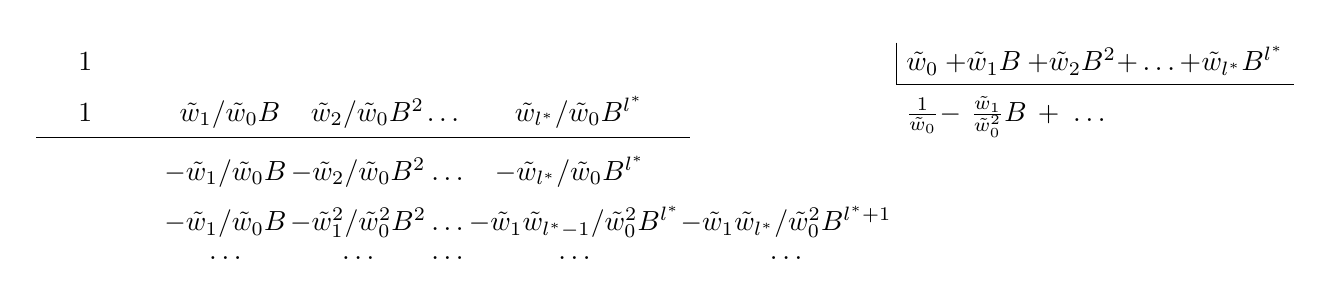
\begin{tikzpicture}
\matrix (a) [matrix of math nodes,column sep=-1.5ex]
{
% x^8 & x^7 & x^6 & x^5 & x^4 &
\phantom{w_1} 1\phantom{ / w_0 B}  & & & & & & & & 
\tilde{w}_0 & +\tilde{w}_1 B & + \tilde{w}_2 B^2 & +  \ldots + & \tilde{w}_{l^*} B^{l^*}\\
\phantom{w_1} 1\phantom{ / w_0 B}& \ \ \tilde{w}_1 / \tilde{w}_0 B \ & \ \ \tilde{w}_2 / \tilde{w}_0 B^2 & 
\ldots \ & \ \tilde{w}_{l^*} / \tilde{w}_0 B^{l^*} & \ & & & 
\frac{1}{\tilde{w}_0} & - \ \frac{\tilde{w}_1}{\tilde{w}_0^2} B & + \ \ldots\\
& -\tilde{w}_1 / \tilde{w}_0 B & -\tilde{w}_2 / \tilde{w}_0 B^2 & \ldots & -\tilde{w}_{l^*} / \tilde{w}_0 B^{l^*} \ \\
& -\tilde{w}_1 / \tilde{w}_0 B & -\tilde{w}_1^2 / \tilde{w}_0^2 B^2 & \ldots & -\tilde{w}_1 \tilde{w}_{l^* - 1} / \tilde{w}_0^2 
B^{l^*} & -\tilde{w}_1 \tilde{w}_{l^*} / \tilde{w}_0^2 B^{l^* + 1} & \phantom{B^l}\\
& \ldots & \ldots & \ldots & \ldots & \ldots \\
};

\draw (a-1-9.north west)|-(a-1-13.south east);
\draw (a-2-1.south west)--(a-4-5.east|-a-2-2.south);
%\draw (a-4-2.south west)--(a-4-6.east|-a-4-4.south);
\end{tikzpicture}

\caption{First 2 terms of polynomial long division}
\label{fig:polyLongDiv}
\end{figure}

\section{Toy Project}
\label{sec:toyProjectFracDiff}
In the previous sections, the \textit{memory vs. stationarity} dilemma has 
been presented. On top of that, through fractional differentiation, 
stationarity has been achieved without totally giving up memory. Also, a 
method has been presented to differentiate and un-differentiate in a robust 
way.\\

That being said, the problem that this toy project attempts to solve will be 
presented. Given a time series $y_t$, and $\Lambda_t$ representing all the 
values $y_t$ has taken up to time $t$, the aim of forecasting is to give a 
prediction $\widehat{y}_{t + 1}$ given $\Lambda_t$. By sequentially giving 
1-day forecasts, a new time series will be generated.\\

To illustrate the effect fractional differentiation can have in the 
predicting power of a model, two models will be designed. One will have 
fully differentiated features and labels, and the other will use 
fractionally differentiated ones.\\

The last phase of the toy project will be computing prediction errors to 
compare the performance of the two models. 

\subsection{Synthetic data}
Striving to create a log-prices time series with memory, the generation was 
the following:

\begin{equation}
\label{eqn:tSeriesSynthetic}
	y_{t} = \frac{1}{5} \cdot \sum_{i = 1}^{5} y_{t - i} + 
	\mu + \epsilon_t \ \ (t \geq 6)
\end{equation}

where $\mu = 0.005$, $\epsilon_t \sim N(0,\ \sigma = 0.01)$ and 
$y_{1:5} = \{0.000,\ 0.075,\ 0.150,\ 0.225,\ 0.300\}$.\\

As it can be seen from the equation \ref{eqn:tSeriesSynthetic}, in order to 
determine the value of $y_t$, it is crucial to know the preceding 5 values 
of the time series. Consequently, if ``memory is erased'', the prediction 
power will decrease. That is, the fractional differentiated time series 
instance at time $t - 1$ will contain more information from the preceding 
days than the fully differentiated series of log-returns.\\

As for the length of the time series, $y_t$ will have 3000 observations, and 
15\% of them (450 obs.) will be saved for testing purposes.

\subsection{Fractional differentiation of $y_t$}
In figure \ref{fig:FFDSynthetic} and \ref{fig:FFDSyntheticZoom} the 
differentiated time series are shown. Note that the method used is the one 
defined previously: fixed-width window fractional differentation method 
(FFD). Also, in order to determine the minimnum $d^*$ that makes the time 
series stationary, figure \ref{fig:ADFSynthetic} and table 
\ref{tab:ADFStatistics} are presented (only training data has been used).\\

\begin{figure}[htbp]
\centering
\begin{minipage}{.5\textwidth}
  \centering
  \includegraphics[scale=0.25]{"\homeCTwo/img/FFDSynthetic"}
  \caption{FFD of $y_t$ - $\tau = 1e-4$}
  \label{fig:FFDSynthetic}
\end{minipage}%
\begin{minipage}{.5\textwidth}
  \centering
  \includegraphics[scale=0.25]{"\homeCTwo/img/FFDSyntheticZoom"}
  \caption{FFD of $y_t$ (Zoomed in) - $\tau = 1e-4$}
  \label{fig:FFDSyntheticZoom}
\end{minipage}
\end{figure}

\begin{figure}[htbp]
\centering
	\includegraphics[scale=0.5]{"\homeCTwo/img/ADFSynthetic"}
	\caption{ADF Statistics of $y_t^d$ - Train}
	\label{fig:ADFSynthetic}
\end{figure}

\begin{table}[htbp]
\centering
	\caption{ADF Test (with trend and drift) Statistics of $y_t^d$ - Train}
	\label{tab:ADFStatistics}
	\vspace{.1cm}
	\begin{tabular}{ |C{2cm}|C{2.5cm}|C{2cm}| }
		\hline
		d & Lag order ($p$) & ADF Statistic\\
		\hline
		0.00 & 13 & -3.130\\
		0.05 & 12 & -3.130\\
		0.10 & 12 & -3.430\\
		0.15 & 12 & -3.850\\
		0.20 & 12 & -4.254\\
		0.25 & 12 & -4.856\\
		0.30 & 12 & -5.352\\
		0.35 & 13 & -6.179\\
		0.40 & 13 & -6.939\\
		0.45 & 13 & -7.525\\
		0.50 & 13 & -8.141\\
		0.55 & 13 & -8.967\\
		0.60 & 13 & -9.819\\
		0.65 & 13 & -10.637\\
		0.70 & 13 & -11.515\\
		0.75 & 13 & -12.388\\
		0.80 & 13 & -13.265\\
		0.85 & 13 & -13.944\\
		0.90 & 13 & -14.684\\
		0.95 & 13 & -15.410\\
		1.00 & 13 & -16.077\\		
		\hline
	\end{tabular}
\end{table}	

Thus, now that it is known that $d^* = 0.2$, whenever the FFD time series is 
mentioned, the order of differentiation will be $d^*$.

\subsection{Models}
With the purpose of evaluating how FFD works in this toy project, three 
models will be used:

\begin{enumerate}
	\item \textbf{Naive Model} (Benchmark): Simplest model than can be 
	built. It will predict $\widehat{y}_{t+1} = y_t$
	\item \textbf{FFD Model:} It will use $y_t^{d^*}$ to predict $y_t$.
	\item \textbf{Returns Model:} It will use $y_t^{1} = y_t - y_{t-1}$ to 
	predict $y_t$.
\end{enumerate}

The FFD and Returns models will be similar in the sense that will use the 
same artificial neural network (ANN) structure and features. The former will 
use a fully-connected hidden layer with 4 units and an output unit (see 
figure \ref{fig:fracDiffANN}), both 
with ELU (Exponential Linear Unit) as activation function.\\

Respecting the features, since the last 5 values have been used to determine 
the next one, that is what will be used. Clarifying:

\begin{itemize}
	\item \textbf{Features:} $y_{t-5}^d$, $y_{t-4}^d$, $y_{t-3}^d$, 
	$y_{t-2}^d$ and $y_{t-1}^d$
	\item \textbf{Labels:} $y_{t}^d$
\end{itemize}

Lastly, recall that 450 observations out of 3000 will be used for testing 
purposes. This does not mean that 2550 observations will be used for 
training, since using the FFD method implies that the series will not be 
defined up to a point because all observations should have the same amount 
of memory (if this did not happen, the first observation would have zero 
memory while the subsequent ones would have more).

\subsection{Sequential forecasts}
\label{sec:toyProjectSeqForecast}
Considering that one is attempting to predict log-prices and differentiated 
features are being used, an emphasis should be put in the 
un-differentiation, which can be expressed (see equation
\ref{eqn:series2Poly}) as:

\begin{equation*}
y_t = \sum_{k = 0}^{T - 1} c_k \cdot B^k (y_t^d) \hspace{.5cm} (T = 3000)
\end{equation*}

Noting $n_0$ as the time stamp where predictions start, the predicted time 
series will be defined sequentially as:

\begin{equation*}
	z_t = \sum_{k = 1}^{T - 1} c_k \cdot B^k (y_t^d) + c_0 \cdot 
	\widehat{y}_t^d \hspace{.5cm} (t \geq n_0)
\end{equation*}

\subsection{Results}
In the previous section, it has been shown how to obtain a new time series 
with the predictions. In order to compare the final time series in the test 
data set ($t \geq n_0$), three metrics will be used: Root-mean-square error 
(RMSE), Mean absolute percentage error (MAPE) and Median absolute deviation 
(MAD). The metrics mentioned will be defined after introducing the following 
parameters: $e_k = y_k - \widehat{y}_k$ and $\tilde{e} = 
\text{median}(e_k)$.

\begin{equation*}
	\text{RMSE} = \sqrt{\frac{\sum_{k = n_0}^{T} (e_k)^2}
	{T - n_0 + 1}} 
\end{equation*}

\begin{equation*}
	\text{MAPE} = \frac{1}{T - n_0 + 1} \cdot \sum_{k = n_0}^T 
	\left| \frac{e_k}{y_k} \right| 
\end{equation*}

\begin{align*}
	\text{MAD} = \text{median}(|e_k - \tilde{e}|)	
\end{align*}

With the metrics defined, the results in the test data set are the 
following:

\begin{table}[htbp]
\centering
	\caption{Error metrics of the models considered - Test}
	\label{tab:MetricsToy}
	\vspace{.1cm}
	\begin{tabular}{ |C{2.5cm}|C{2.5cm}|C{2.5cm}|C{2.5cm}| }
		\hline
			 & FFD model & Naive model & Returns model\\
		\hline
		RMSE & 0.010184 & 0.012995 & 0.013126\\
		MAPE & 0.001608 & 0.002113 & 0.002148\\
		MAD  & 0.006606 & 0.008747 & 0.009192\\		
		\hline
	\end{tabular}
\end{table}

\begin{figure}[htbp]
\centering
	\includegraphics[scale=0.25]{"\homeCTwo/img/errorMetricsToy"}
	\caption{Error metrics of the models considered - Test}
	\label{fig:MetricsToy}
\end{figure}

\subsection{Conclusions}
From the results shown in table \ref{tab:MetricsToy} and figure 
\ref{fig:MetricsToy}, it can be implied that the FFD model has performed 
best across all error metrics. Also, the difference between the Naive and 
Returns Model is negligible, so it can be concluded that the Returns Model 
has not been able to detect the pattern behind the observations.\\

This goes to say that fractionally differentiating the data provides much 
information in a much clearer way than full differentiation. In other words, 
even tough the original time series can be reconstructed with both methods, 
the FFD method provides information with memory without having to do any 
transformation.\\

The next step is to apply the same method to a real financial time series. 
Although this controlled project has been successful in an FFD sense, it 
remains to be seen whether memory in financial time series helps with 
forecasts.

\section{Financial data}
\label{sec:fracDiffFinData}
The data used will be the \textbf{log-prices} of the S\&P500 from 2005-01-01 
to 2019-09-01. It will include the Open ($y_t^{\text{Open}}$), High 
($y_t^{\text{High}}$), Low ($y_t^{\text{Low}}$) and Close 
($y_t^{\text{Close}}$). That is, the log-price it opens/closes and the 
highest/lowest values during the daily trading session.\\

As in the project of section \ref{sec:toyProjectFracDiff}, the goal of the 
models will be to make a 1-day forecast. In particular, with the OHLC (Open 
High, Low, Close) data of day $t$, the models will predict the value the 
stock closes at time $t + 1$. To do that, the features and labels 
will be the following:

\begin{itemize}
	\item \textbf{Features:} $y_t^{\text{Open}}$, $y_t^{\text{High}}$, 
	$y_t^{\text{Low}}$ and $y_t^{\text{Close}}$
	\item \textbf{Labels:} $y_{t + 1}^{\text{Close}}$
\end{itemize}

These features have been chosen because they provide information at 
different times of the day. That is, they represent the daily state of the 
time series, and thus, having memory could provide and advantage, since 
comparisons between them could be made.

\subsection{Division Train/Test data sets}
The data will be divided into a training and test data set. The distribution 
is the following:

\begin{table}[htbp]
	\centering
	\caption{Division of Train/Test}
	\label{tab:trainTestFracDiff}
	\vspace{.1cm}
	\begin{tabular}{ |C{3.5cm}|C{2.5cm}|C{2.5cm}| }
		\hline
			 				& FFD model & Returns model\\
		\hline
		Start date (Train)	& 2006-10-06 & 2005-01-04\\
		End date (Train)		& 2017-07-12 & 2017-07-12\\
		\hline
		Start date (Test)	& 2017-07-14 & 2017-07-14\\
		End date (Test)		& 2020-08-28 & 2020-08-28\\
		\hline
		$n_{\text{Train}}$	& 2709 		 & 3152\\
		$n_{\text{Test}}$	& 788  		 & 788\\		
		\hline
	\end{tabular}
\end{table}

As it can be seen in table \ref{tab:trainTestFracDiff}, both the FFD and the 
Returns models have 788 observations in the test data set. However, in the 
train data set, the FFD has approximately 450 fewer observations. This can 
be explained via equation \ref{eqn:FFD}, since by \textbf{setting a 
threshold} $\tau = 1e-4$, an $l^*(\tau, d)$ exists such that the FFD is 
valid for $t \geq l^* +1$. In particular, in the case of returns $d = 1$, 
and thus, $l^*(\tau, d = 1) = 1$ since the first observation does not have a 
preceding value.\\

Also note that $n_{\text{Test}}$ has been kept equal because the error 
metrics will be evaluated in this data set. Consequently, the conditions 
should be the same to avoid misleading results.

\section{Models}
As in section \ref{sec:toyProjectFracDiff}, three models will be used: 
\textbf{Naive}, \textbf{FFD} and \textbf{Returns} model. The features will 
be the corresponding time series shown in section \ref{sec:fracDiffFinData}, 
but differentiated. To be specific, the FFD model will use the fractionally 
differentiated features with the minimum order ($d^* = 0.25$) that makes the 
4 OHLC time series stationary (in training). Conversely, the 
\textbf{Returns} model will use fully differentiated features ($d = 1$).\\

The \textbf{FFD} and \textbf{Returns} models will use an ANN with the 
structure seen in figure \ref{fig:fracDiffANN}. As in section 
\ref{sec:toyProjectFracDiff}, the activation function will be the 
Exponential Linear Unit (ELU).

\begin{figure}[htbp]
	\centering
	\includegraphics{"\homeCTwo/img/fracDiffANN"}
	\caption{ANN used in the FFD and Returns Models}
	\label{fig:fracDiffANN}
\end{figure}

\section{Data normalization}
As a means to provide features to the neural network with the same range, 
all 4 features have been normalized:

\begin{equation*}
	z_t = \frac{y_t - y_{\text{min}}}{y_{\text{max}} - y_{\text{min}}}
\end{equation*}

It should be pointed out that $y_{\text{max}}$ and $y_{\text{min}}$ have 
been computed in the \textbf{train} data set. It is extremely important to 
consider this, because if one were to use the maximum/minimum of the whole 
data set, look-ahead bias would have occurred. To be more specific, if the 
test observations started at time $t_0$ and the time stamp when the maximum 
is achieved is $t_0 + m > t_0$, then the forecast at time $t_0$ would have 
used information from $t_0 + m$, which is impossible.\\

That being said, in the train data set, $z_t \in [0, 1]$, while in the test 
data set, features are not guaranteed to be in $I = [0, 1]$. However, 
working under the assumption that the complete time series is stationary, 
values can not be far off.\\

It should be brought up that since labels are not normalized, the predicted 
values will not have to undergo ``un-normalization''.

\section{Results}
\label{sec:resultsFFD}
As in section \ref{sec:toyProjectSeqForecast}, the sequential forecasts have 
been calculated and the final result is 3 time series, which are forecasts 
of the close of the S\&P500:

\begin{align*}
	y_t^{\text{Naive}} \hspace{.51cm} (n_0 + 1 \leq t \leq T)\\
	y_t^{\text{FFD}} \hspace{.64cm} (n_0 + 1 \leq t \leq T)\\
	y_t^{\text{Returns}} \hspace{.25cm} \hfill (n_0 + 1 \leq t \leq T)\\
\end{align*}

Where $t = n_0$ is the time stamp that marks the start of the test data set. 
Therefore, the prediction will be of the value of the log-price close of 
$t + 1 = n_0 + 1$\\

\begin{table}[htbp]
\centering
	\caption{Error metrics of the models considered - Test}
	\label{tab:MetricsFFD}
	\vspace{.1cm}
	\begin{tabular}{ |C{2.5cm}|C{2.5cm}|C{2.5cm}|C{2.5cm}| }
		\hline
			 & FFD model 	& Naive model 	& Returns model\\
		\hline
		RMSE & 0.0187200 	& 0.0185758 		& 0.0181539\\
		MAPE & 0.0017909 	& 0.0017573 		& 0.0017179\\
		MAD  & 0.0047790 	& 0.0044728 		& 0.0044403\\		
		\hline
	\end{tabular}
\end{table}


In table \ref{tab:MetricsFFD} and figure \ref{fig:MetricsFFD} the error 
metrics for the three models considered are shown. In addition, in figures 
\ref{fig:resultsFFD1}, \ref{fig:resultsFFD2} and \ref{fig:resultsFFD3} the 
forecasted time series are presented for different periods of time.

\begin{figure}[htbp]
	\centering
	\begin{minipage}{.5\textwidth}
  		\centering
		\includegraphics[scale=0.25]{"\homeCTwo/img/errorMetricsFFD"}
		\caption{Error metrics of the models considered - Test}
		\label{fig:MetricsFFD}
	\end{minipage}%
	\begin{minipage}{.5\textwidth}
  		\centering
		\includegraphics[scale=0.25]{"\homeCTwo/img/resultsFFD1"}
		\caption{Forecasted time series - Test}
		\label{fig:resultsFFD1}
	\end{minipage}
\end{figure}


\begin{figure}[htbp]
	\centering
	\begin{minipage}{.5\textwidth}
  		\centering
  		\includegraphics[scale=0.25]{"\homeCTwo/img/resultsFFD2"}
  		\caption{Results 2018-07/2018-10}
  		\label{fig:resultsFFD2}
	\end{minipage}%
	\begin{minipage}{.5\textwidth}
  		\centering
  		\includegraphics[scale=0.25]{"\homeCTwo/img/resultsFFD3"}
  		\caption{Results 2019-03/2019-06}
  		\label{fig:resultsFFD3}
	\end{minipage}
\end{figure}

\section{Conclusions}
As it was shown in section \ref{sec:resultsFFD}, 

\bibliography{references}
% PDFLaTeX + MakeIndex + BibTeX

\end{document}
 
